%%-------------------------------------------------------------------------------------- Início
\section{Configuração do Heroku}
\begin{frame}[allowframebreaks,fragile,t]{Implantação da aplicação Rails}
  \begin{enumerate}
    \item Registre um usuário no Heroku \url{http://www.heroku.com}.
    \begin{figure}[h!]
	\centering
	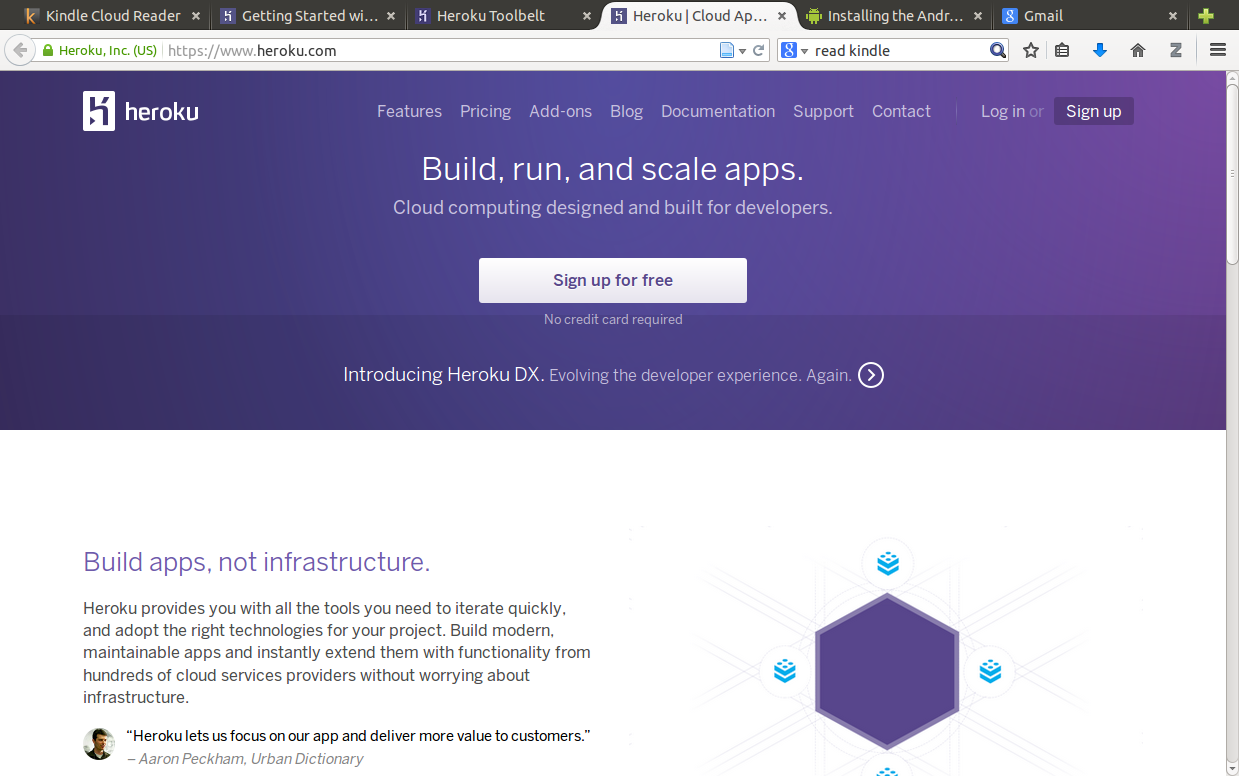
\includegraphics[width=0.60\textwidth]{devops/imagens/heroku-1.png}
    \end{figure}
 
 \framebreak
    \item Clique no botão \verb!Sign up for free!, forneça seu e-mail e clique no botão
      \verb!Sign up!.
    \begin{figure}[h!]
	\centering
	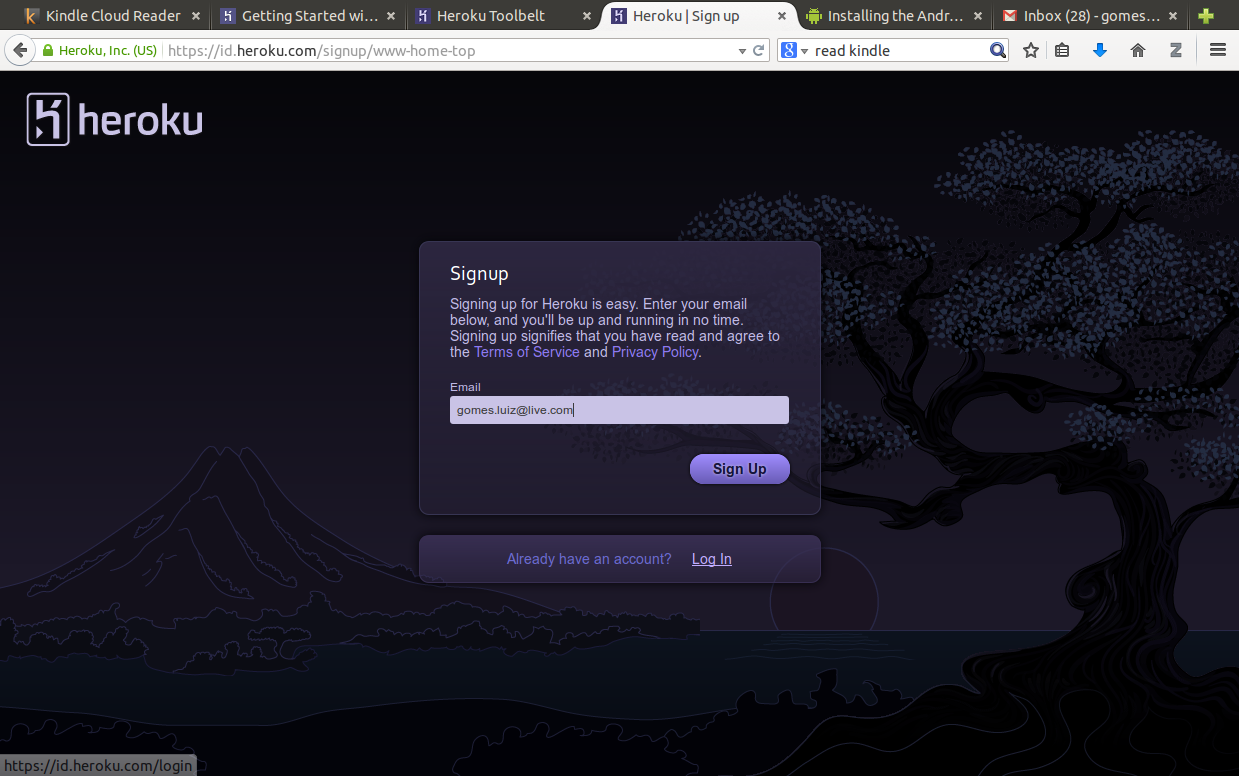
\includegraphics[width=0.60\textwidth]{devops/imagens/heroku-2.png}
    \end{figure}

 \framebreak
    \item Conecte-se ao servidor de e-mail informado e confirme o registro do usuário.
    \begin{figure}[h!]
	\centering
	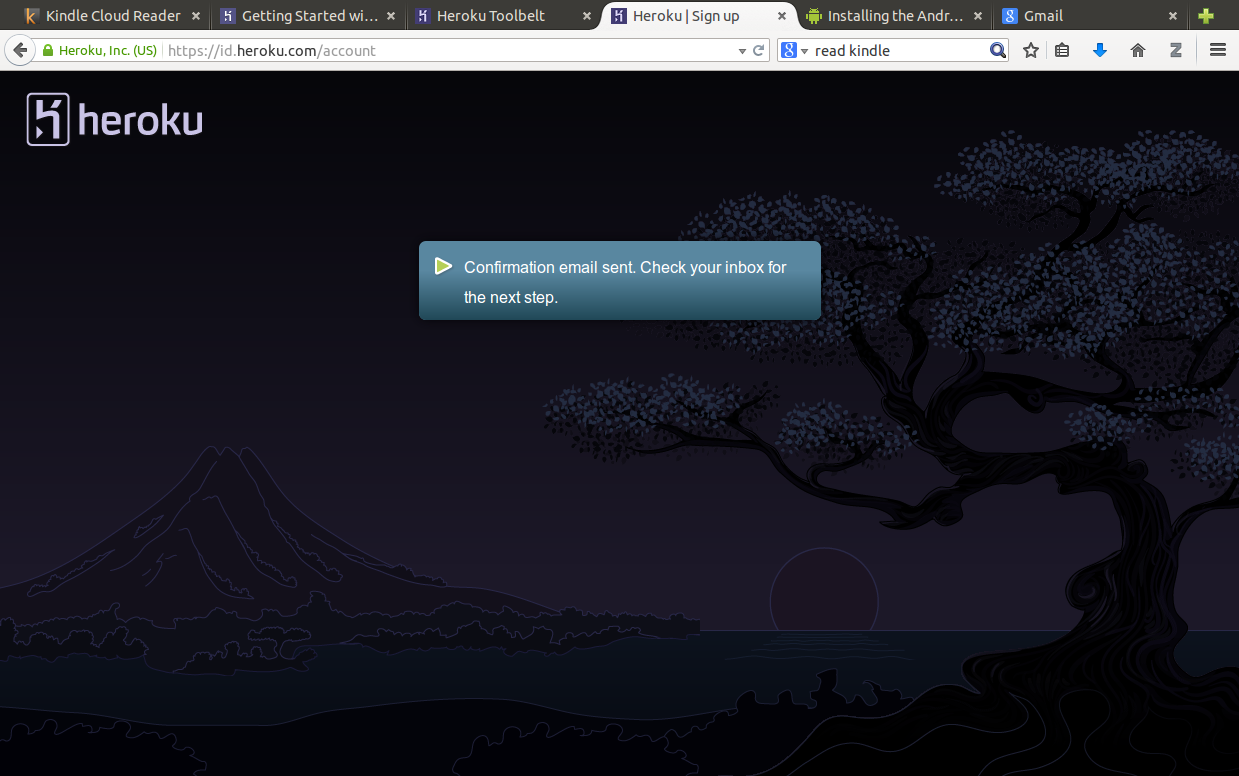
\includegraphics[width=0.60\textwidth]{devops/imagens/heroku-3.png}
    \end{figure}
 
 \framebreak
    \item Forneça a senha, confirme-a e clique no botão \verb!Save!.
    \begin{figure}[h!]
	\centering
	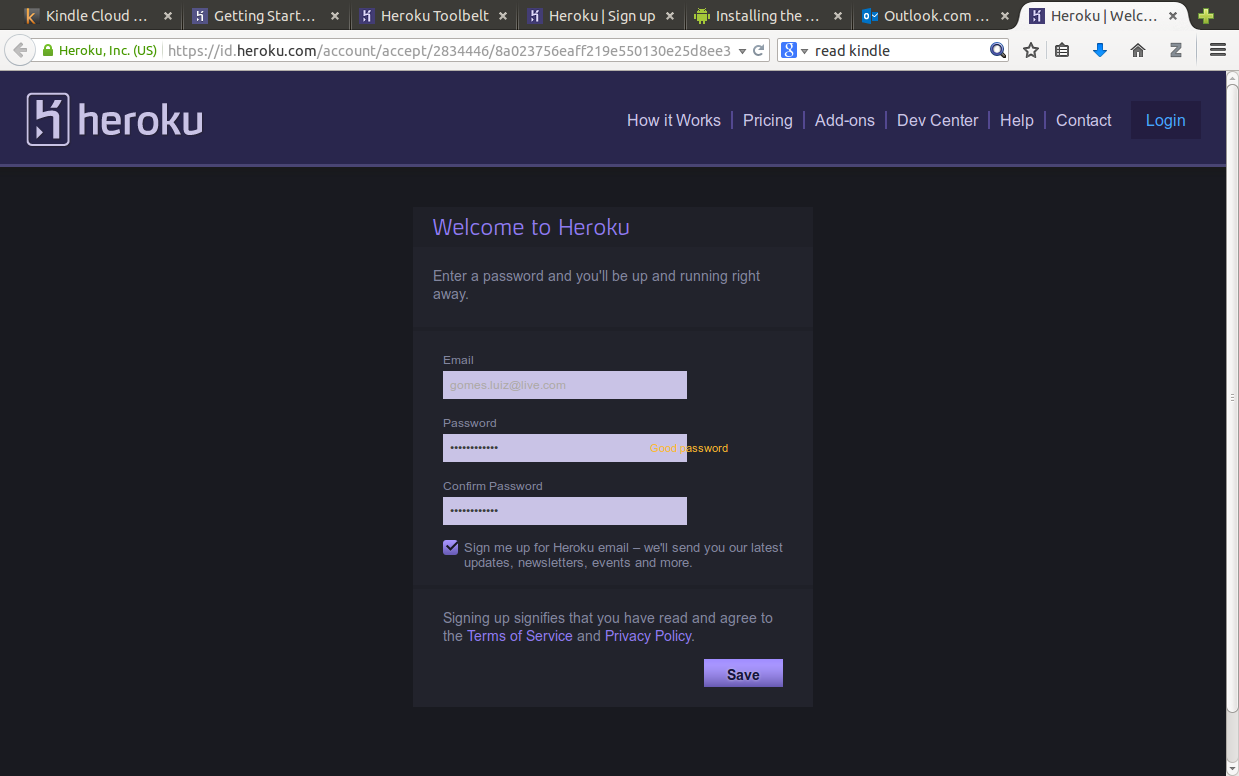
\includegraphics[width=0.60\textwidth]{devops/imagens/heroku-4.png}
    \end{figure}
    
\framebreak
    \item Após isso, se tudo ocorreu corretamente, a seguinte página deverá ser apresentada. 
    \begin{figure}[h!]
	\centering
	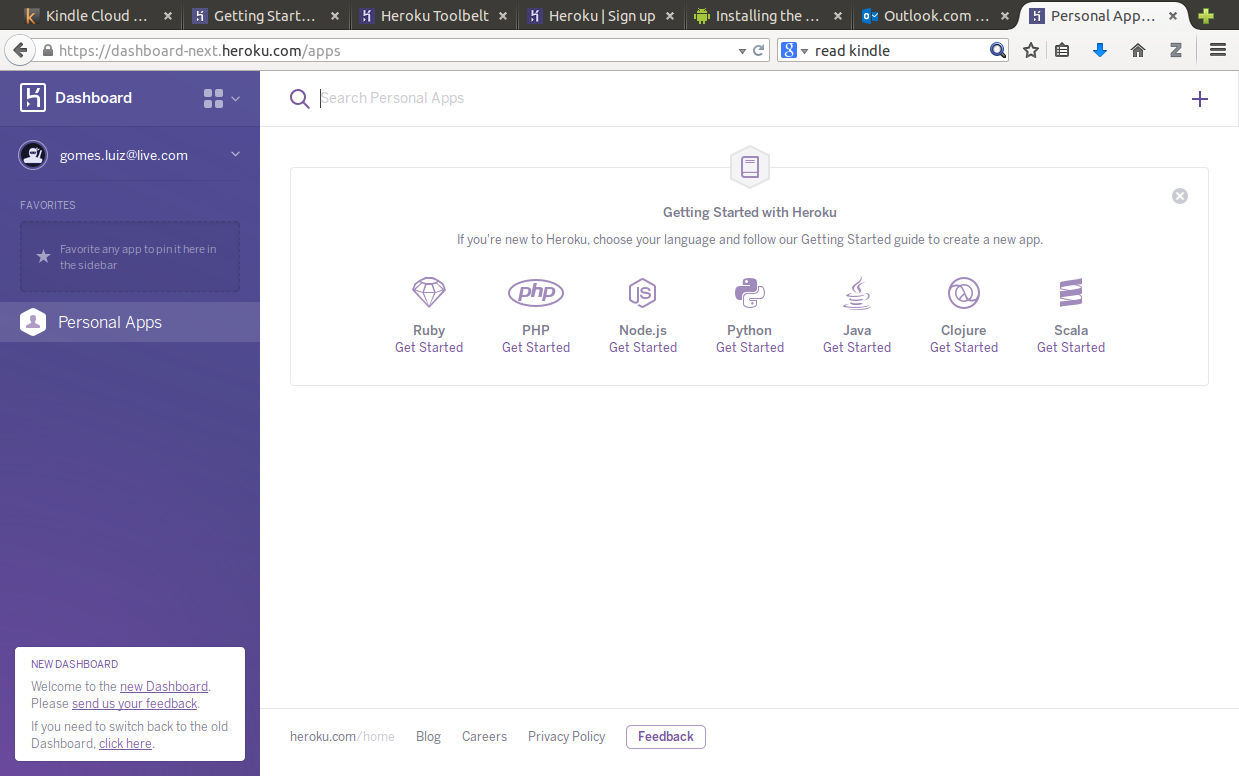
\includegraphics[width=0.60\textwidth]{devops/imagens/heroku-5.png}
    \end{figure}
  
\framebreak
    \item No Gedit, tecle \verb!F9! para que o \alert{Browser de Arquivos} apareça e navegue
      até a pasta \verb!$HOME/Workspace/blog!. 
    \begin{figure}[h!]
	\centering
	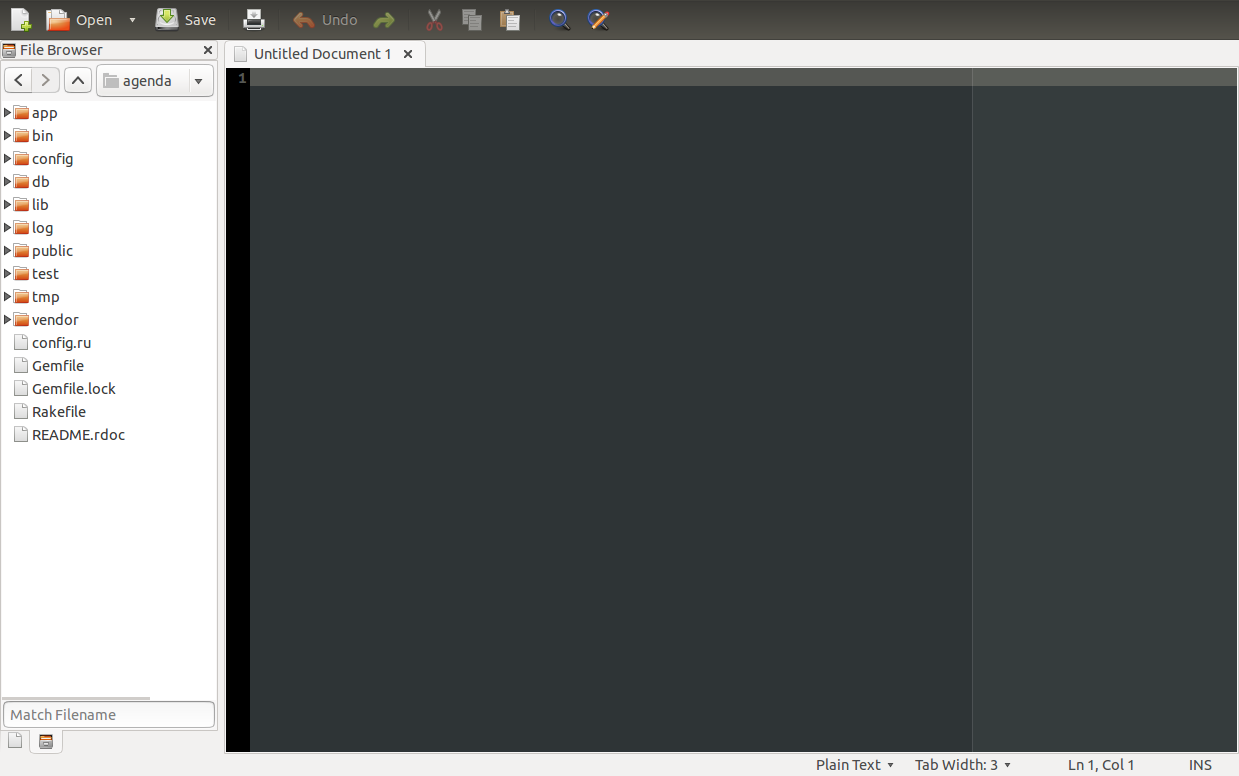
\includegraphics[width=0.60\textwidth]{devops/imagens/gedit-5.png}
    \end{figure}

 \framebreak
    \item  Abra o arquivo \alert{Gemfile} e modifique/acrescente as seguintes linhas, após a 
    a primeira linha \verb!source 'https://rubygems.org'!.
    \begin{lstlisting}[style=BashInputStyle]
      
      # Use o sqlite3 como banco de dados de desenvolvimento e teste.
      group :development, :test do
        gem 'sqlite3'
      end 

      # Use o PostgreeSQL como banco de dados de producao.
      group :production do
			  gem 'pg'
      end 
    \end{lstlisting}     
 \framebreak
 \framebreak
    \item  Instale as bibliotecas necessárias, se elas ainda não foram instaladas
      anteriormente.
    \begin{lstlisting}[style=BashInputStyle]
      $ bundle install --without production
      $ git add .
      $ git commit -am "Heroku config"
    \end{lstlisting}
 
 \framebreak
    %\item  Instale as ferramentas cliente para a criação e gerenciamento de aplicações no Heroku.
    %\begin{lstlisting}[style=BashInputStyle]
		%	$ wget -O- https://toolbelt.heroku.com/install-ubuntu.sh | sh
    %\end{lstlisting}
     
    \item  Conecte-se ao Heroku com suas credenciais (e-mail e senha).
    \begin{lstlisting}[style=BashInputStyle]
      $ heroku login --interactive
      Enter your Heroku credentials.
      Email: ruby@example.com
      Password:
      Could not find an existing public key.
      Would you like to generate one? [Yn] Y
      Generating new SSH public key.
      Uploading ssh public key /Users/adam/.ssh/id_rsa.pub
    \end{lstlisting}

    \item Navegue para a pasta da aplicação Rails, criada na última aula, denominada de \verb!blog!.
    \begin{lstlisting}[style=BashInputStyle]
      cd ~/workspace/blog
      $ heroku create
      Creating polar-inlet-4930... done, stack is cedar
      http://infinite-springs-7216.herokuapp.com/ 
	| git@heroku.com:polar-inlet-4930.git
      Git remote heroku added
    \end{lstlisting}
    
    \item Implante a aplicação nos servidores do Heroku.
    \begin{lstlisting}[style=BashInputStyle]
      $ git push heroku master
      Fetching repository, done.
      Counting objects: 10, done.
      Delta compression using up to 4 threads.
      Compressing objects: 100% (6/6), done.
      Writing objects: 100% (6/6), 876 bytes | 0 bytes/s, done.
      Total 6 (delta 4), reused 0 (delta 0)
    \end{lstlisting}
     
    \item Executa a migração do banco de dados.
    \begin{lstlisting}[style=BashInputStyle]
			$ heroku run rake db:migrate
    \end{lstlisting}
    
    \item Agora abra a aplicação no navegador, a URL é aquela gerada pelo comando
      \verb!heroku create! que, neste caso, é \url{http://infinite-springs-7216.herokuapp.com/}.
    \begin{lstlisting}[style=BashInputStyle]
      $ heroku open
    \end{lstlisting}
    
    \item Renomeie a aplicação para um nome mais amigável. Este nome deverá ser único.
    \begin{lstlisting}[style=BashInputStyle]
      $ heroku apps:rename blog-do-luiz
    \end{lstlisting}
        
  \end{enumerate}
\end{frame}
%%-------------------------------------------------------------------------------------- Início